\documentclass [xcolor=svgnames, t] {beamer} 

\mode<presentation> {
    \usetheme{CambridgeUS}
}
\usepackage{amssymb,amsmath,amsthm,enumerate}
\usepackage{graphicx,animate}
\usepackage{multirow}
\usepackage{bm}
\usepackage{media9}
\usepackage{listings}
\lstset
{
    breaklines=true,
}
\setbeamertemplate{caption}[numbered]
\usepackage[utf8]{inputenc}
\usepackage{booktabs, comment} 
\usepackage[absolute, overlay]{textpos} 
\usepackage{pgfpages}
\useoutertheme{infolines} 

\usepackage{amsmath}
\usepackage[makeroom]{cancel}
\usepackage{textpos}
\usepackage{tikz}
\usepackage[en-US]{datetime2} % to use the date formate Month day, year
\usepackage{hyperref} % to add hyperlink for urls ending in .php
%\DeclareUrlCommand\url{\color{magenta}\def\UrlLeft{https://}\urlstyle{tt}}
\usepackage[font=footnotesize]{caption}
\usepackage{subcaption} % for subfigure
\addtobeamertemplate{footnote}{}{\vspace{2ex}} % lift footnote a bit so that it doesn't collide with the navigation bar

% code listing style here
\definecolor{codegreen}{rgb}{0,0.6,0}
\definecolor{codegray}{rgb}{0.5,0.5,0.5}
\definecolor{codepurple}{rgb}{0.58,0,0.82}
\definecolor{backcolour}{rgb}{0.95,0.95,0.92}

\lstdefinestyle{myTeXstyle}{
    backgroundcolor=\color{backcolour},
    commentstyle=\color{codegreen},
    keywordstyle=\color{magenta},
    numberstyle=\tiny\color{codegray},
    stringstyle=\color{codepurple},
    basicstyle=\ttfamily\footnotesize,
    breakatwhitespace=false,
    breaklines=true,
    captionpos=b,
    keepspaces=true,
    morekeywords={begin},
    language=TeX,
    numbers=left,
    numbersep=5pt,
    showspaces=false,
    showstringspaces=false,
    showtabs=false,
    tabsize=2
}

\lstset{style=myTeXstyle}
% code listing style end

% some meta information
\title[SURE LaTeX Tutorial]{SURE \LaTeX\ Tutorial}
%\subtitle{(Your Sub Title)}
\institute[]{Department of Applied Math  \\Illinois Tech}
\titlegraphic{
\includegraphics[height=2.5cm]{SURE.png}}
\author[Y. Ding, Y. Cheng]{Yuhan Ding, Yuanxing Cheng}
\institute[]{Department of Applied Math  \\Illinois Institute of Technology}
\date{\today}

% navigation bar style
\addtobeamertemplate{navigation symbols}{}{%
    \usebeamerfont{footline}%
    \usebeamercolor[fg]{footline}%
    \hspace{1em}%
    \insertframenumber/\inserttotalframenumber
}

\begin{document}
\begin{frame}
    \maketitle % front page
\end{frame}


%%%%%%%%%%%%%%%%%%%%%%%%%%%%
% add nsf logo from the second page
\logo{
\includegraphics[height=1.0cm]{figures/NSFLOGO.png}~}
%%%%%%%%%%%%%%%%%%%%%%%%%%

\begin{frame}{Outline}
	\tableofcontents[sectionstyle=show,subsectionstyle=show/shaded/hide,subsubsectionstyle=show/shaded/hide] %toc
\end{frame}

\section{Intro To \LaTeX}
\subsection{What is \LaTeX}
\begin{frame}{What is \LaTeX \footnote{From The \LaTeX\ Project Website
            \href{www.latex-project.org}{\texttt{www.latex-project.org}}} }
    \begin{itemize}
        \item A document preparation system
        \item Features designed for the production of technical and scientific documentation
        \begin{itemize}
            \item mathematical equations
            \item cross referencing
            \item tons of packages to meet different needs
        \end{itemize}
        \item De facto standard for the communication and publication of scientific documents
        \item An open-source software (\alert{free!!!})
        \item \alert{NOT} What-You-See-Is-What-You-Get
    \end{itemize}
\end{frame}

\begin{frame}{One example}
    \begin{figure}
        \centering
        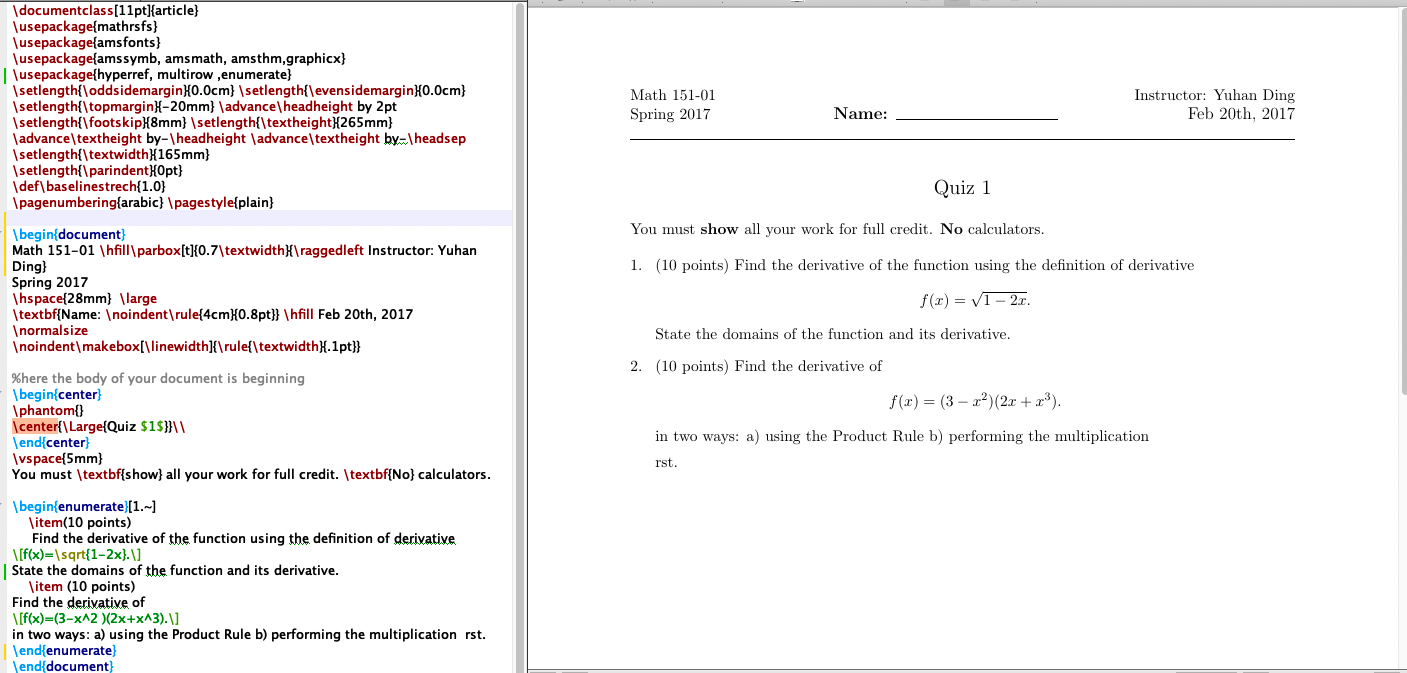
\includegraphics[width = 0.90\textwidth]{figures/inputoutput.png}
        \caption{Using \LaTeX\ to create a quiz. The left part is what you see/type and the right part is what you get.}
    \end{figure}
\end{frame}

\subsection{What is \LaTeX\ used for}
\begin{frame}{What is \LaTeX\ Used for}
    \begin{figure}
        \centering
        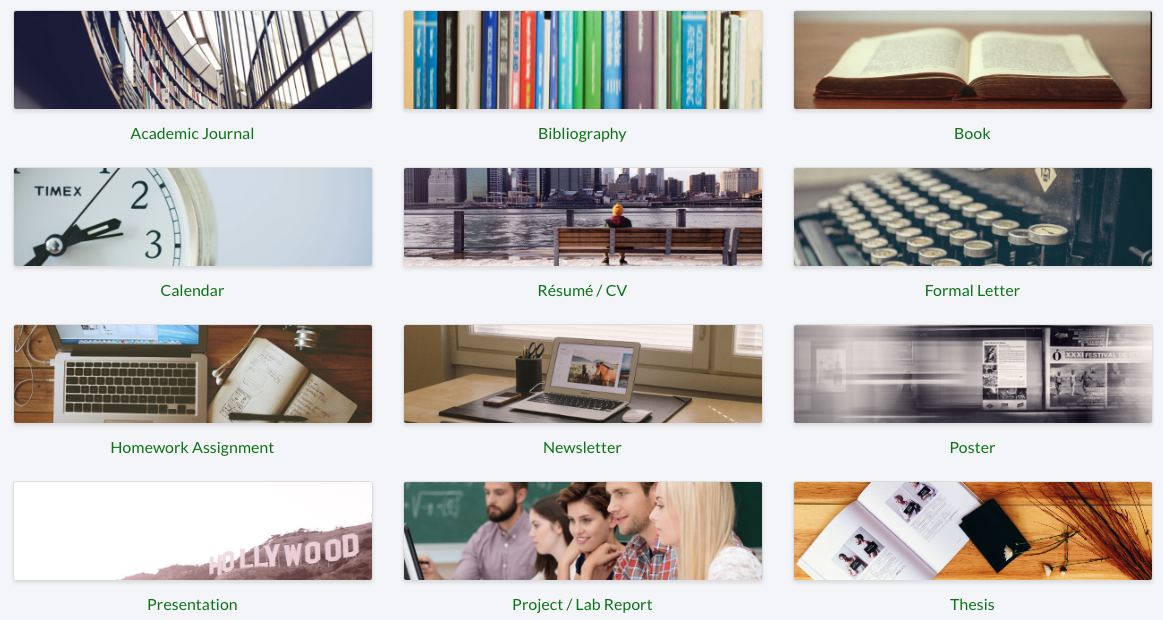
\includegraphics[width = 0.90\textwidth]{figures/Templates.png}
        \caption{Various \LaTeX\ projects. \href{https://www.overleaf.com/latex/templates}{Source: Overleaf templates}}
    \end{figure}
\end{frame}

\subsection{How to Access}
\begin{frame}{Resources}
    \begin{itemize}
        \item TeX system: TeXLive, \url{www.tug.org/texlive/}
        \item Online compiling tools
        \begin{itemize}
            \item Equation Editor: \href{https://latexeditor.lagrida.com/}{\texttt{latexeditor.lagrida.com}}
            \item OverLeaf (Recommended): \url{www.overleaf.com}
        \end{itemize}
        \item Offline compiling tools
        \begin{itemize}
            \item VS Code + \href{{https://github.com/James-Yu/LaTeX-Workshop/wiki/Install}}{\LaTeX\ Workshop Extension}
            \item TeXStudio: \url{www.texstudio.org}
            \item All in one portable version: \href{https://github.com/symera/TexPortable}{TeXPortable} (Windows only)
            \item Real-time compiling: \href{www.texifier.com}{TeXifier} (Mac, iOS only) (not free)
        \end{itemize}
        \item Other tutorials
        \begin{itemize}
            \item \href{https://tug.org/levels.html}{The levels of TeX}
            \item \href{http://mirrors.ctan.org/info/latex-doc-ptr/latex-doc-ptr.pdf}{A First Set of \LaTeX\ Resources}
            \item \href{https://www.overleaf.com/learn}{Overleaf documentation}
            \item \href{https://www.colorado.edu/aps/latex-primer}{\LaTeX\ for Beginners with TeXworks}
            \item \href{https://guides.nyu.edu/LaTeX}{NYU Libraries \LaTeX\ guides}
        \end{itemize}
    \end{itemize}
\end{frame}
\begin{frame}{Software Interface}
    \begin{columns}
        \begin{column}{.45\textwidth}
            \vspace*{-1em}
            \begin{figure}
                \centering
                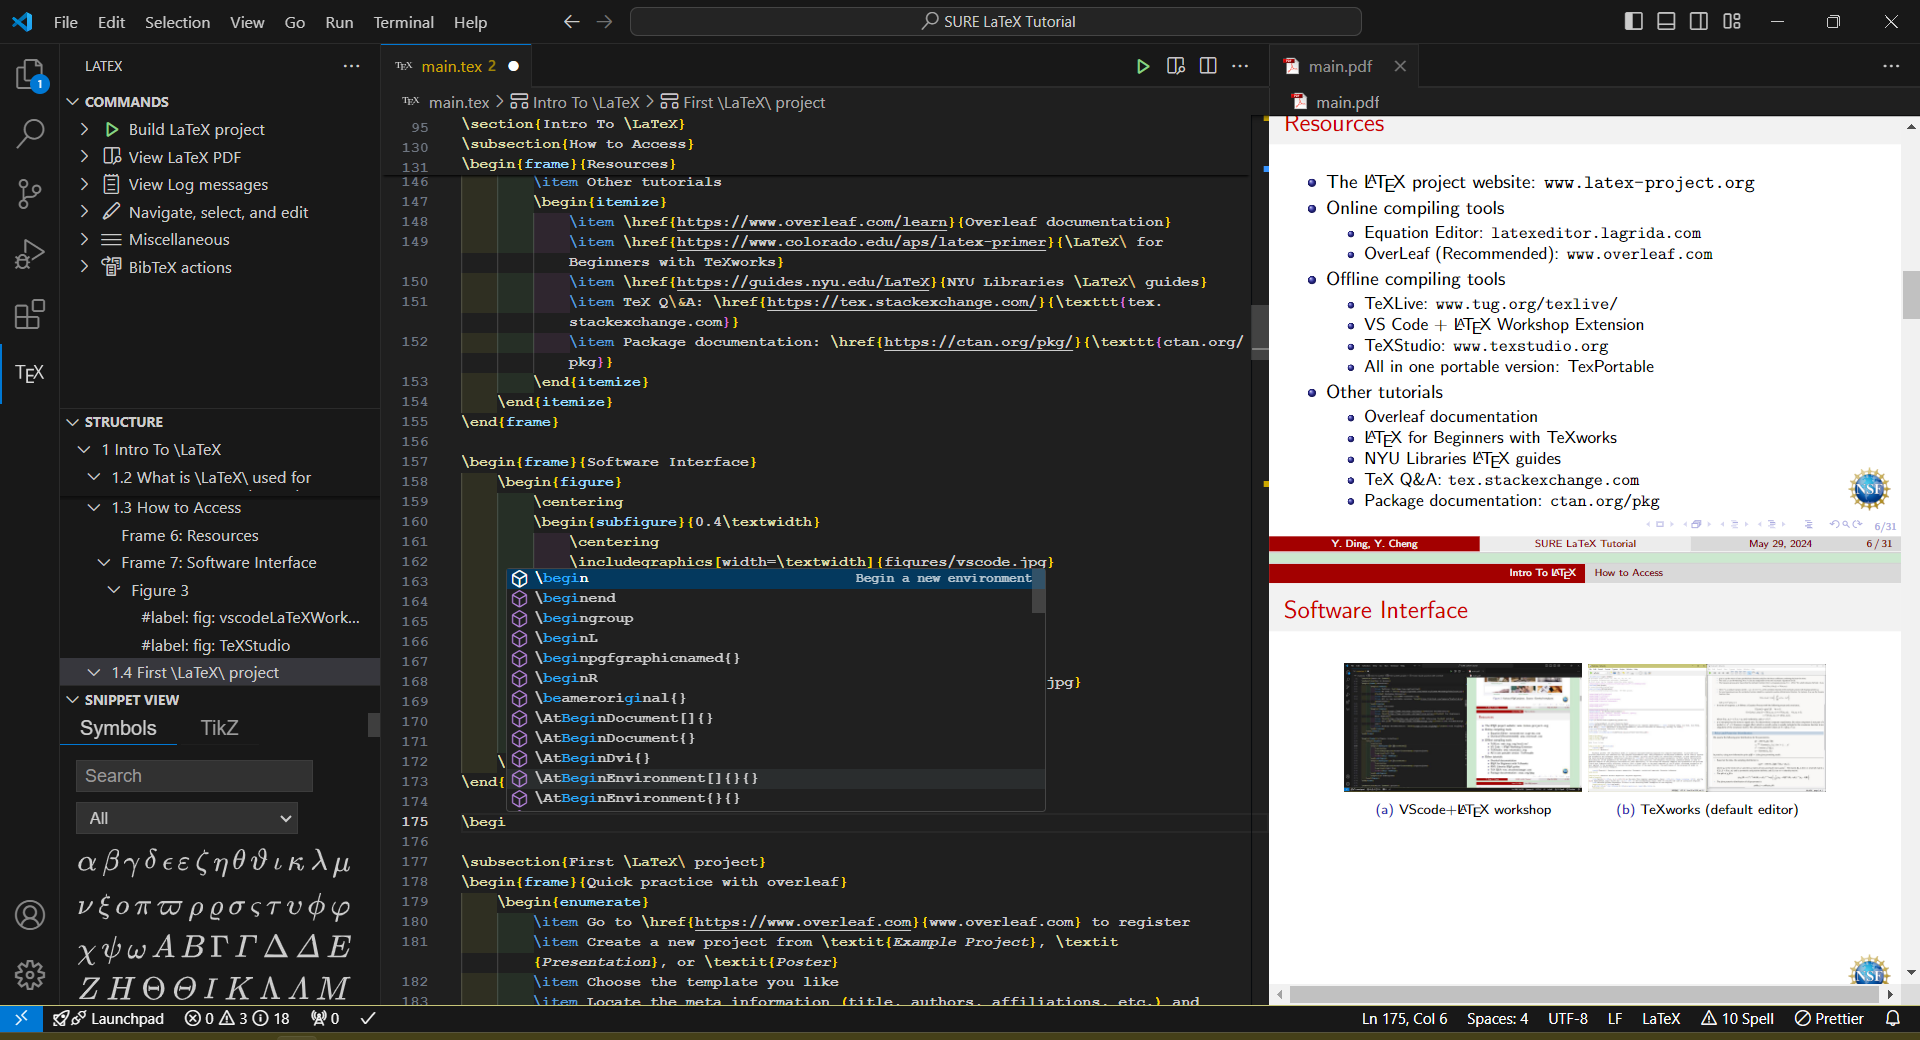
\includegraphics[width=\textwidth]{figures/vscode}
                \caption{VScode+\LaTeX\ workshop}
                \label{fig: vscodeLaTeXWorkshop}
            \end{figure}
            \vspace*{-1em}
            \begin{itemize}
                \item modern interface
                \item smart completions 
                \item extensible and customizable
            \end{itemize}
        \end{column}
        \begin{column}{.45\textwidth}
            \vspace*{-1em}
            \begin{figure}
                \centering
                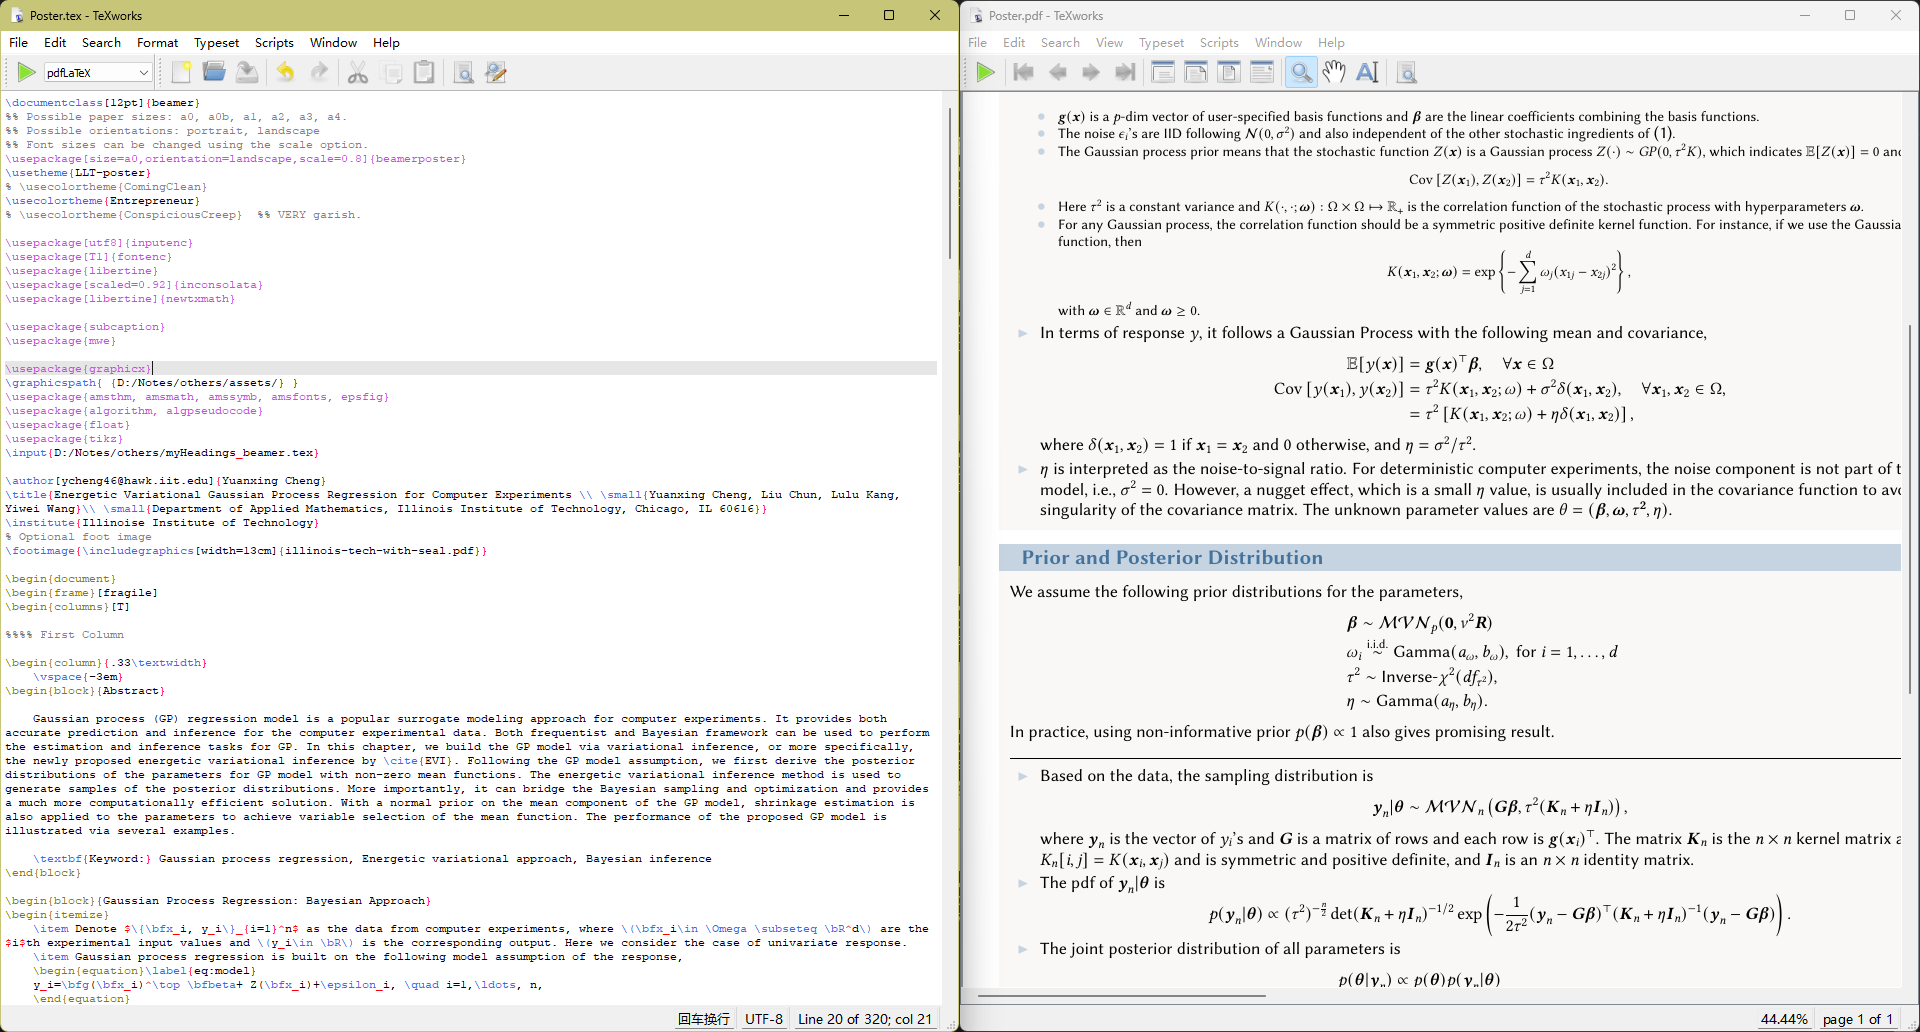
\includegraphics[width=\textwidth]{figures/texstudio}
                \caption{TeXworks (default editor)}
                \label{fig: TeXStudio}
            \end{figure}
            \vspace*{-1em}
            \begin{itemize}
                \item comes with TeXLive
                \item fast, clean and simple
            \end{itemize}
        \end{column}
    \end{columns}
\end{frame}

\subsection{First \LaTeX\ project}
\begin{frame}{Quick practice with overleaf}
    \begin{enumerate}
        \item Go to \href{https://www.overleaf.com}{www.overleaf.com} to register
        \item Create a new project from \textit{Example Project}, \textit{Presentation}, or \textit{Poster}
        \item Choose the template you like
        \item Locate the meta information (title, authors, affiliations, etc.) and change them accordingly.
        \item Make a title in the first page.
        \item Write something in the main page. Change the font of some words. Then generate some dummy text.
    \end{enumerate}
    You can open the beamer template used in Overleaf guide via \href{https://www.overleaf.com/project/new/template/19345?id=65231945}{this link}. Some codes about the title page to try out \href{https://en.wikibooks.org/wiki/LaTeX/Title_Creation}{here}.
\end{frame}

\section{Tips to start your first \LaTeX\ project}
\begin{frame}[fragile]{Tips}
    \begin{itemize}
        \item Start from a template (presentation and poster)
            \begin{itemize}
                \item Overleaf templates:
                    \href{https://www.overleaf.com/latex/templates}{\texttt{www.overleaf.com/latex/templates}}
                \item more LaTeX templates: \href{https://www.latextemplates.com}{\texttt{www.latextemplates.com}}
            \end{itemize}
        \item Use \verb|%| to add comments
        \item \LaTeX\ macros format: \verb|\command[options]{args}{args}{...}|
        \begin{itemize}
            \item \verb|{\color{red}{red text}}| gives {\color{red}{red text}}
            \item \verb|\textit{italic text}| gives \textit{italic text}
            \item \verb|\usepackage{amssymb}| to load commands defined in package \texttt{amssymb}
        \end{itemize}
        \item Paired \LaTeX\ macros format: \verb|\begin[options]{macro} ... \end{macro}|
        \item Hit Tab key to auto complete macro in the first hint
        \item Use Google or ChatBot to search solutions
    \end{itemize}
\end{frame}


\subsection{Mathematical Symbols}
\begin{frame}{How to type mathematical symbols}
    \begin{itemize}
        \item Need to load package \texttt{amssymb}
    \end{itemize}
    \begin{figure}
        \centering
        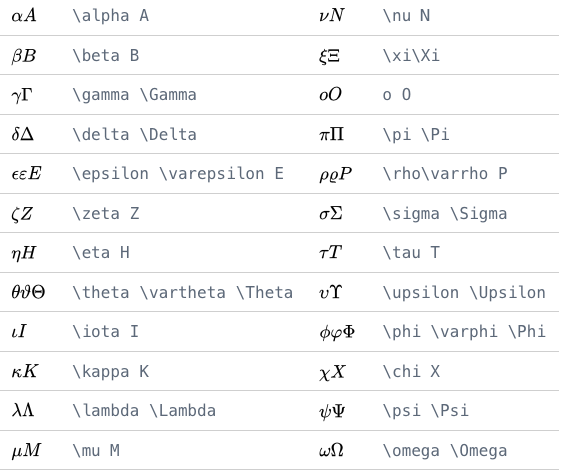
\includegraphics[height = 50mm]{figures/GreekLetters.png}
        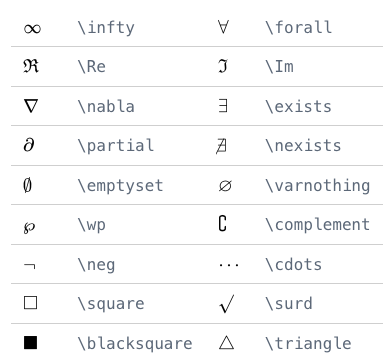
\includegraphics[height = 50mm]{figures/mathsymbol.png}
    \end{figure}

    You can find more details via \href{https://www.overleaf.com/learn/latex/List_of_Greek_letters_and_math_symbols}{this link}.
\end{frame}

\subsection{inline and display math}
\begin{frame}[fragile]{Example}
    Input:\\
    \begin{lstlisting}
Use paired dollar sign for inline math formula $\int_0^2 \frac{\sqrt{x^2+1}}{x+1} \, dx$ and \[ ... \] for display math formula. For example, 
\[ \int_0^2 \frac{\sqrt{x^2+1}}{x+1} \, dx \]\end{lstlisting}
    Output:\\
    Use paired dollar sign for inline math formula $\int_0^2 \frac{\sqrt{x^2+1}}{x+1} \, dx$ and \textbackslash[ ... \textbackslash] for display math formula. For example, 
    \[ \int_0^2 \frac{\sqrt{x^2+1}}{x+1} \, dx \]
\end{frame}

\begin{frame}{Some macros}
    \vspace*{-2em}
    \begin{center}
        \begin{tabular}{ll}\\ \hline
            code & usage \\ \hline
            \texttt{\textbackslash circ} & $\circ$, function composition \\
            \texttt{\textbackslash text\{\}}, \texttt{\textbackslash textrm\{\}} & display text in equation\\
            \texttt{\textbackslash texttt\{\}} & show as typeset font\\
            \texttt{\textbackslash displaystyle} & change inline style to display style \\
            \texttt{\textbackslash nolimits} & change limits placement \\
            \texttt{\textbackslash,}, \texttt{\textbackslash:}, \texttt{\textbackslash;}, \texttt{\textbackslash quad} & some white space \\ 
            \texttt{\textbackslash max} & max operator, e.g. $\max_{x\in A}$ \\
            \texttt{\textbackslash left( \textbackslash right)} & parenthesis auto 
            resized\\ 
            \texttt{\textbackslash begin\{equation\}} & to number and reference the equation\\
            \texttt{\textbackslash label\{tag\}} & to add a tag to the equation\\
            \texttt{\textbackslash ref\{tag\}}, \texttt{\textbackslash eqref\{tag\}} & to refer to the content with the tag\\
            \texttt{\textbackslash begin\{cases\}} & to define piecewise function in equation\\
            \texttt{\textbackslash\textbackslash} & to start from new line in piecewise \\
            \texttt{\&} & to align equations in piecewise \\
            \hline
        \end{tabular}
    \end{center}
\end{frame}

\begin{frame}[fragile]{Practice}
    Try to type the following. You can start from \href{https://latexeditor.lagrida.com/}{this online tool}.
    \[ \sum_{n=1}^\infty \frac{1}{n^2}= \frac{\pi^2}{6}\]
    \begin{equation*}
        y=\begin{cases}
            x+5, & x>3\\
            x-5, & x<=3
        \end{cases}
    \end{equation*}
    \begin{equation} \label{eqn:exampleEqn}
        f(x) = \frac{1}{\sigma \sqrt{2\pi}} e^{-\frac{1}{2}\left(\frac{x-\mu}{\sigma}\right)^2}
    \end{equation}
    Equation \eqref{eqn:exampleEqn} is the general form of a normal distribution's probability density function. By default, equations are auto numbered. Use the star variant \verb|\begin{equation*}| or simply \textbackslash[ ... \textbackslash] to avoid numbering.
\end{frame}

\subsection{alignment}
\begin{frame}[fragile]{How to align several equations}
    \vspace{-0.5em}
    Input:\\
    \vspace{-0.2em}
    \begin{lstlisting}
\begin{equation}\label{eqn:exampleOpt}
    \begin{split}
        \min_{x\geq 2} &\qquad x^2+5x+6+y\\
        s.t. &\qquad x+y=5
    \end{split}
\end{equation}\end{lstlisting}
    \vspace{-0.2em}
    Output:
    \vspace{-0.2em}
    \begin{equation}\label{eqn:exampleOpt}
        \begin{aligned}
            &\min_{x\geq 2} & x^2+5x+6+y\\
            &s.t. & x+y=5
        \end{aligned}
    \end{equation}
    \vspace{-0.2em}
    In this way the whole equation is numbered as a block. To use multiple alignment, use \verb|\begin{align*}| and number with the method mentioned \href{https://tex.stackexchange.com/a/42728}{here}.  More examples can be found in \href{https://docs.aspose.com/tex/java/latex-structures-for-equations/}{this website}, and \href{https://en.wikibooks.org/wiki/LaTeX/Advanced_Mathematics#Vertically_aligning_displayed_mathematics}{this website}.
\end{frame}

\begin{frame}{Practice}
    Try a few examples from above mentioned websites and type the following.
    \begin{align*}
        (a+b)^2 &= c^2+4\times \frac{ab}{2}\\
        a^2 + 2ab+b^2&= c^2+2ab\\
        a^2 + b^2 &= c^2
    \end{align*}
    \begin{equation*}
        \left(\begin{aligned}
            f(x) && g(y) && h(z)\\
            1 && 2 && 3\\
            4 && 5 && 6
        \end{aligned}\right)
    \end{equation*}
\end{frame}

\subsection{Insert Figures}
\begin{frame}[fragile]{How to insert a figure}
    \begin{lstlisting}
\begin{figure}
    \centering
    
\includegraphics[width = 0.3 \textwidth]{figures/pamu.jpeg} 
    \caption{\label{fig:pom} My Figure} 
\end{figure}\end{lstlisting}
    \begin{figure}
        \centering
        
\includegraphics[width = 0.3 \textwidth]{figures/pamu.jpeg}
        \caption{\label{fig:pom} My Figure}
    \end{figure}
\end{frame}

\begin{frame}[fragile]{How to put multiple figures together}
    Input:
    \begin{lstlisting}
\begin{figure}
    \centering
    \begin{subfigure}{0.3\textwidth}
        \centering
        
\includegraphics[width=\textwidth]{figures/pamu}
        \caption{left fig caption}
        \label{fig: subfig1}
    \end{subfigure}
    \begin{subfigure}{0.3\textwidth}
        \centering
        
\includegraphics[width=\textwidth]{figures/pamu}
        \caption{right fig caption}
        \label{fig: subfig2}
    \end{subfigure}
    \caption{2 subfigures}
\end{figure}\end{lstlisting}
\end{frame}

\begin{frame}
    Output: 
    \begin{figure}
        \centering
        \begin{subfigure}{0.3\textwidth}
            \centering
            
\includegraphics[width=\textwidth]{figures/pamu}
            \caption{left fig caption}
            \label{fig: subfig1}
        \end{subfigure}
        \begin{subfigure}{0.3\textwidth}
            \centering
            
\includegraphics[width=\textwidth]{figures/pamu}
            \caption{right fig caption}
            \label{fig: subfig2}
        \end{subfigure}
        \caption{2 subfigures}
    \end{figure}

    Also try to use .pdf as image format to have the best image quality. Say in Python matplotlib, you can use $\texttt{plt.savefig('figure.pdf')}$.
\end{frame}

\begin{frame}[fragile]{How to refer a figure}
    \begin{itemize}
        \item Input
        \begin{lstlisting}
If you want to refer to the figure, you can type Fig \ref{fig:pom} to refer to the figure with number.\end{lstlisting}
        \item Output: If you want to refer to the figure, you can type Fig \ref{fig:pom} to refer to the figure with number.
        \item Note: In the beamer document, you need to add the following command to show the figure numbers. \verb|\setbeamertemplate{caption}[numbered]|
        \item Practice: Please insert a figure into your practice project, and include a caption for a short description. Then refer it in the next paragraph.
        \item Find more details on \href{https://www.overleaf.com/learn/how-to/Including_images_on_Overleaf}{including images on Overleaf}.
    \end{itemize}
\end{frame}

\subsection{Insert Tables}
\begin{frame}[fragile]{How to insert tables}
        Input:
        \begin{lstlisting}
\begin{table}
    \centering
    \begin{tabular}{l|r|c}
        No. & Item & Quantity \\ \hline
        1 & Widgets & 42 \\
        2 & Gadgets & 13
        \end{tabular}
    \caption{\label{tab:widgets}An example table.}
\end{table}
\end{lstlisting}
        Output:
        \begin{table}
            \centering
            \begin{tabular}{l|r|c}
                No. & Item    & Quantity \\
                \hline
                1   & Widgets & 42       \\
                2   & Gadgets & 13
            \end{tabular}
            \caption{\label{tab:widgets}An example table.}
        \end{table}
\end{frame}

\begin{frame}[fragile]{Combining rows}
        Input: (Require \texttt{multirow} package)
        \begin{lstlisting}
\begin{center} % to put the table in the center of the page
    \begin{tabular}{ |c|c|c| } \hline
        col1 & col2 & col3 \\ \hline
        \multirow{3}{4em}{Multiple row} & cell2 & cell3 \\ 
        & cell5 & cell6 \\ 
        & cell8 & cell9 \\ 
        \hline
    \end{tabular}
\end{center}
\end{lstlisting}
        Output:
        \begin{center}
            \begin{tabular}{ |c|c|c| }
                \hline
                col1                            & col2  & col3  \\
                \hline
                \multirow{3}{4em}{Multiple row} & cell2 & cell3 \\
                                                & cell5 & cell6 \\
                                                & cell8 & cell9 \\
                \hline
            \end{tabular}
        \end{center}
\end{frame}

\begin{frame}[fragile]{Combining columns}

        Input:
        \begin{lstlisting}
\begin{tabular}{ |p{2cm}||p{1cm}|p{1cm}|} \hline 
    \multicolumn{3}{|c|}{Country List} \\ \hline 
    Country or Area Name & ISO ALPHA 2 Code & ISO Numeric Code\\ \hline
    Afghanistan & AF & 004\\ \hline
\end{tabular}
\end{lstlisting}
        Output (without centering):\\
        \begin{tabular}{ |p{2cm}||p{1cm}|p{1cm}|}
            \hline
            \multicolumn{3}{|c|}{Country List}                         \\
            \hline
            Country or Area Name & ISO ALPHA 2 Code & ISO Numeric Code \\
            \hline
            Afghanistan          & AF               & 004              \\
            \hline
        \end{tabular}
\end{frame}

\begin{frame}[fragile]{Practice}
    \begin{table}
        \centering
        \begin{tabular}{ |c|c|c|c|c|c|c| }
            \hline
            \multicolumn{7}{|c|}{Table of Brownian Motions}                                   \\
            \hline
            \multirow{3}{2em}{For Fun} & $j$      & 0 & 1       & 2       & 3       & 4       \\
            & $t_j$    & 0 & 1/12    & 1/6     & 1/4     & 1/3     \\
            & $B(t_j)$ & 0 & -0.1730 & -0.3552 & -0.1735 & -0.3473 \\
            \hline
        \end{tabular}
        \caption{Practice Table1
            \label{tab:practable1}}
    \end{table}
    \vspace{-1em}
    The next table is from normal distribution \href{https://en.wikipedia.org/wiki/Normal_distribution}{wikipedia page}. The multiline equation inside table/tabular can be typed in \verb|\begin{array}|.
    \begin{table}
        \centering
        \begin{tabular}{l|l} \hline
            Notation & $\mathcal{N}(\mu,\sigma^2)$\\ \hline
            Parameters & \hspace*{-0.5em}$\begin{array}{l}
                \mu \in \mathbb{R}\\
                \sigma^2 \in \mathbb{R}_{>0}
            \end{array}$\\ \hline
            Support & $x\in\mathbb{R}$ \\\hline
        \end{tabular}
        \caption{Practice Table2\label{tab:practable2}}
    \end{table}
    \vspace{-1em}
    More information on \href{https://www.overleaf.com/learn/latex/tables}{Overleaf guides}.
\end{frame}

\section{How to cite}
\subsection{References}
\begin{frame}[fragile]{Citation and references}
    \begin{enumerate}
        \item Prepare \verb|your-bib.bib| file used to store bibTeX entries.
        \begin{lstlisting}
@article{greenwade93,
author  = "George D. Greenwade",
title   = "The {C}omprehensive {T}ex {A}rchive {N}etwork ({CTAN})",    year    = "1993",
journal = "TUGBoat",
volume  = "14",
number  = "3",
pages   = "342--351"}\end{lstlisting}
        \item Specify a bibliography style in the .tex file: \verb|\bibliographystyle{alpha}|
        \item Use \verb|\cite{citation-key1, citation-key2}| to cite the paper in the documents. e.g. \cite{greenwade93}, \cite{AFCIP,ITDS}.
        \item Use \verb|\bibliography{your-bib}| to generate a reference section including all cited entries
    \end{enumerate}
\end{frame}

\begin{frame}[fragile]{How to get .bib file}
    \begin{itemize}
        \item start from a blank text file and change the file extension to .bib
        \item copy the bibTeX entries (Google scholar, Semantic scholar, BibItNow, etc.), or generated using reference management software
        \begin{itemize}
            \item Zotero, with browser addon: \url{www.zotero.org}
            \item bibDesk (Mac only) \href{bibdesk.sourceforge.io}{\texttt{bibdesk.sourceforge.io}}
            \item Mendeley
        \end{itemize}
    \end{itemize}
    \begin{figure}
        \centering
        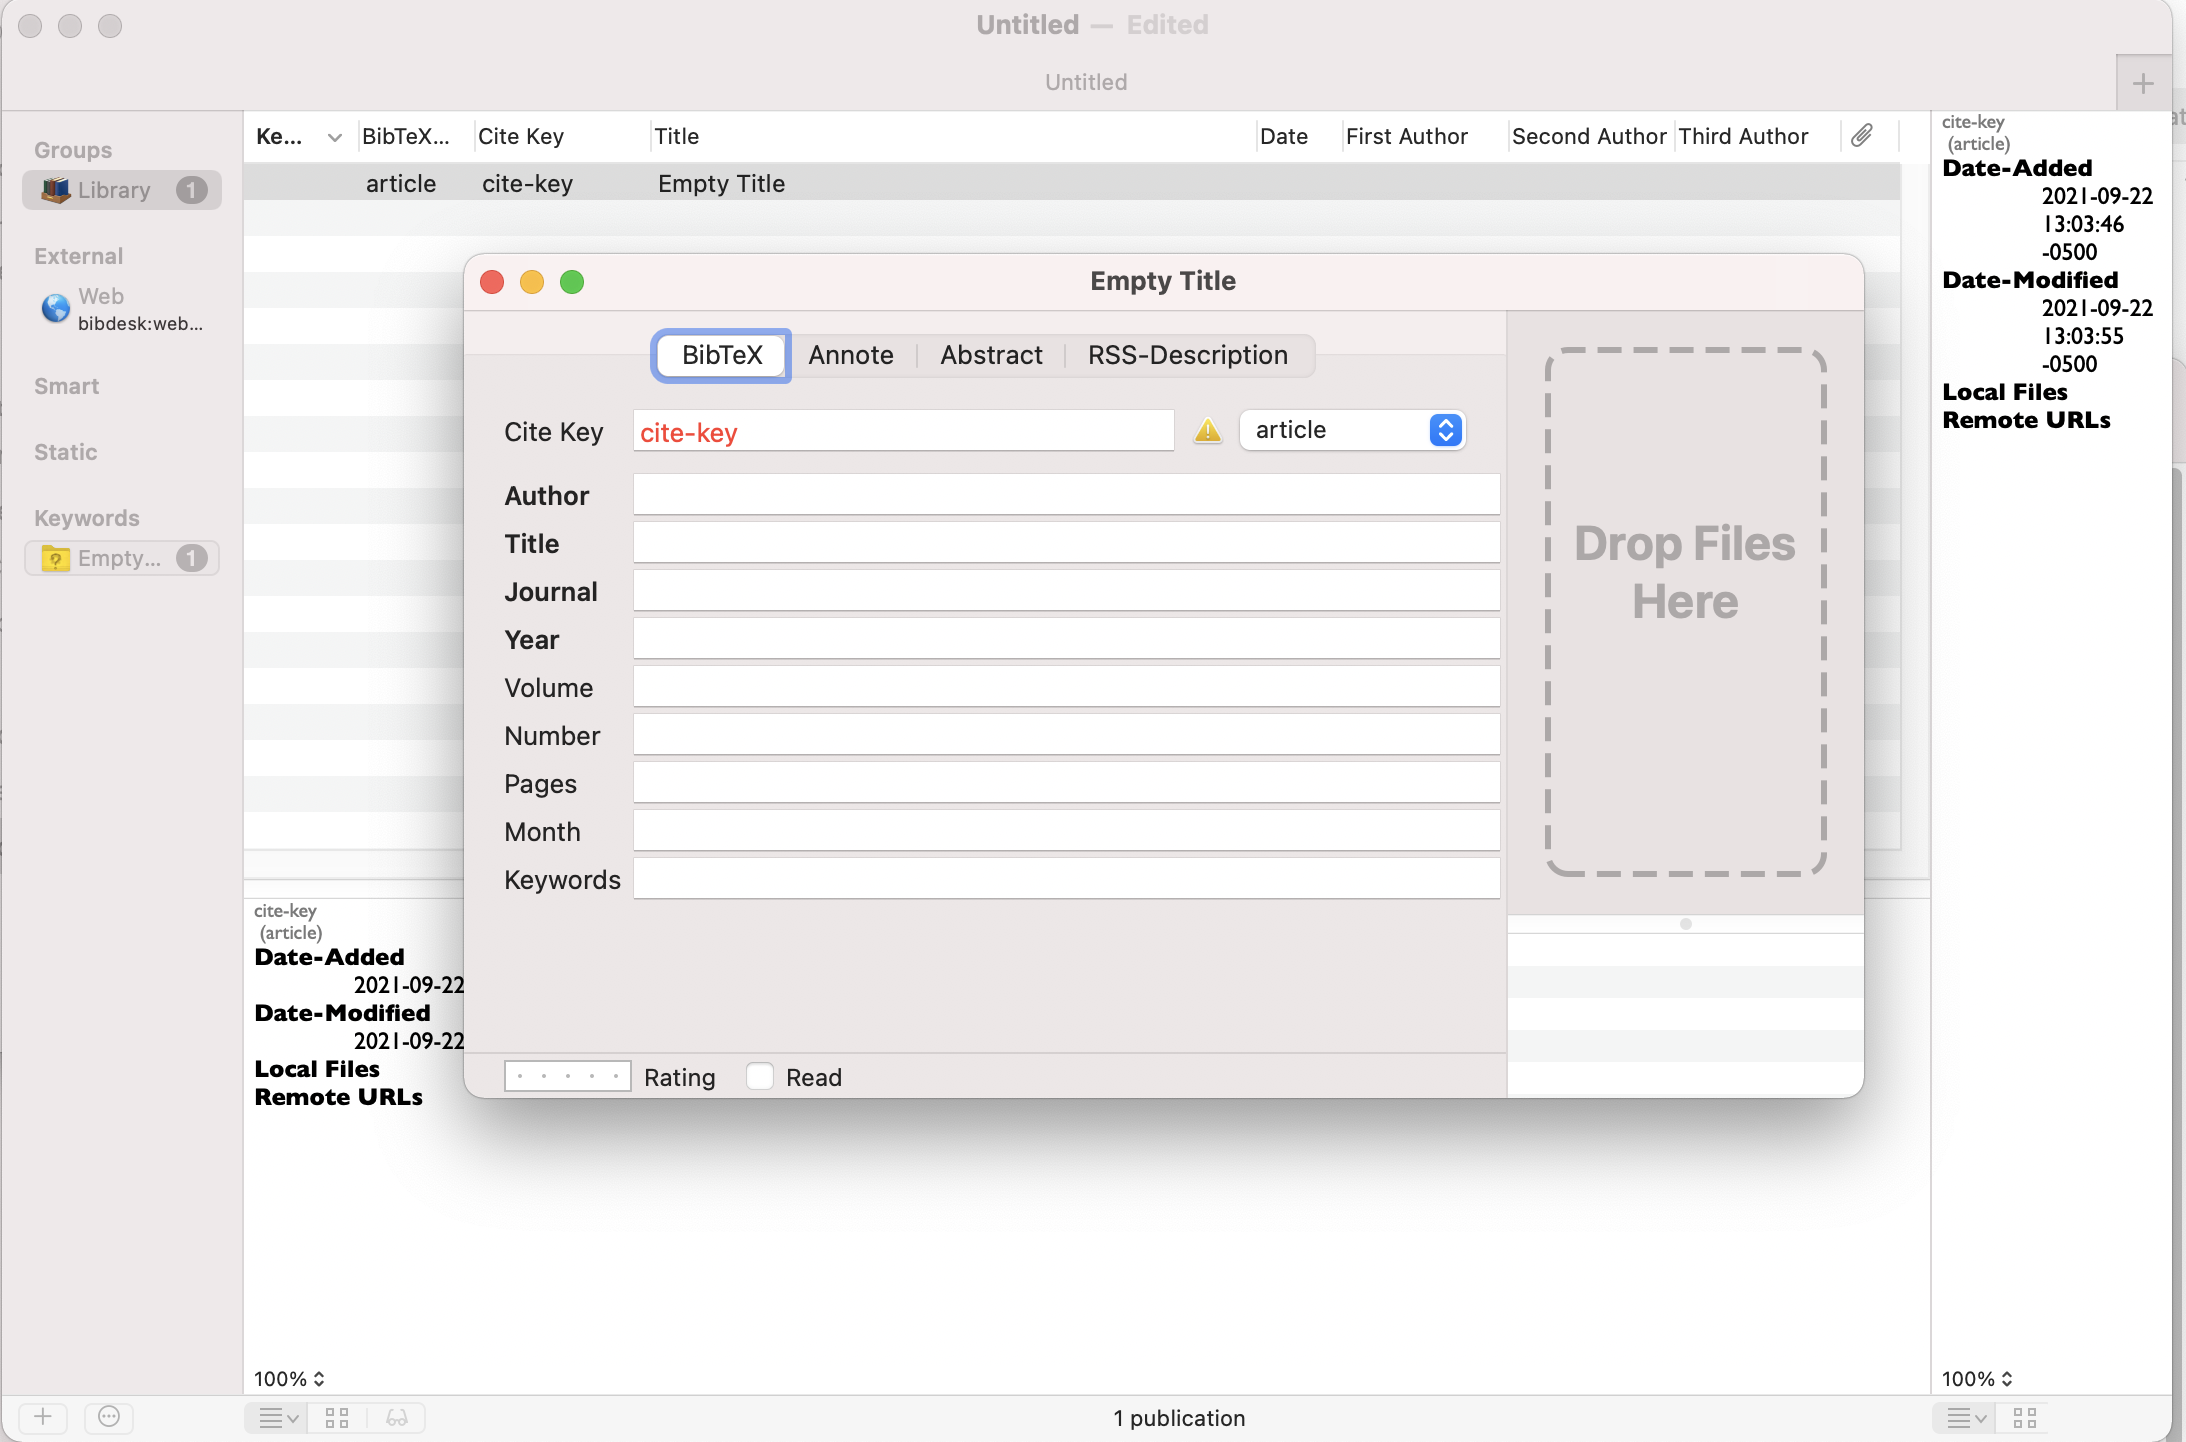
\includegraphics[width = 0.4 \textwidth]{figures/BibDesk.png}
        \caption{bibDesk interface}
    \end{figure}
\end{frame}

\begin{frame}{Practice}
    \begin{enumerate}
        \item obtain your own .bib file
        \item add one or two bibTeX entries
        \item upload it to overleaf, or put it in the same folder with your .tex file
        \item cite the paper in your .bib file
        \item add a reference page in the end of your document
    \end{enumerate}
\end{frame}

\section{Tips to finish your first \LaTeX\ project}
\subsection{Debugging}
\begin{frame}[fragile]{How to debug?}
    \begin{itemize}
        \item Check whether commands are in pair or not. e.g., \verb|\begin \end \[ \] { }|
        \item Check missing \& and \verb|\\| in table
        \item Read the error messages carefully
        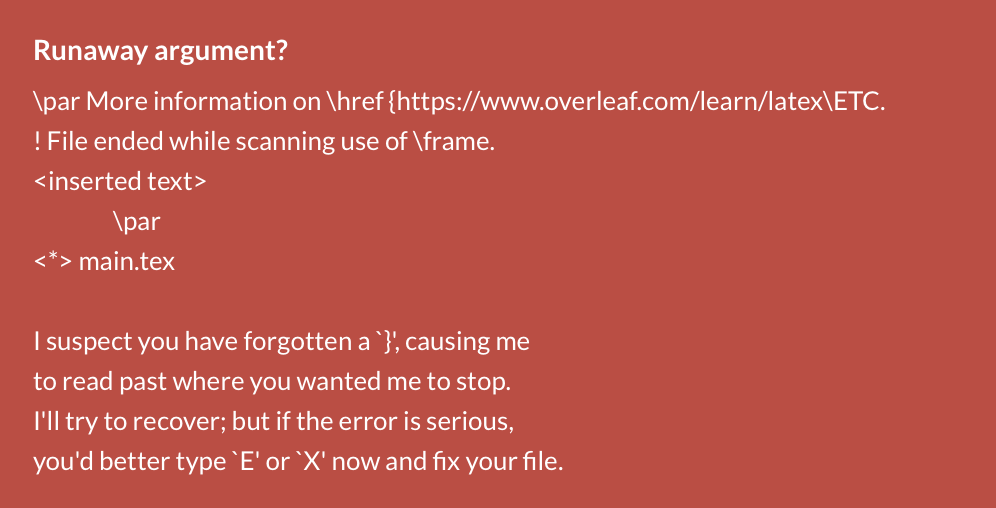
\includegraphics[height = 40mm]{figures/ErrorMessages.png}
        \item Syntax error reminder in OverLeaf
        
\includegraphics[width = 50mm]{figures/ErrorIndicator.png}
    \end{itemize}
\end{frame}

\subsection{Almost Done}
\begin{frame}[fragile]{Minor adjustments}
    \begin{itemize}
        \item check output to see if anything missing (successful but incomplete compiling)
        \item check typos
        \item use inverse search to locate the tex source code from the pdf. For example in LaTeXWorkshop
        \begin{itemize}
            \item option "jump to source"
            \item ctrl + click: from pdf to tex
            \item ctrl + alt + j: both way
        \end{itemize}
        \item use \verb|\vspace{1mm}|, \verb|\hspace{-0.5em}|, etc. to adjust spacing
        \item adjust figure size to avoid overlapping of document elements
        \item make a backup
    \end{itemize}
\end{frame}

\section{Tips on using Beamer}
\begin{frame}[fragile]{What is Beamer}
    \vspace{-1em}
    \begin{center}
        \verb|\documentclass[options]{beamer}|\\
    \end{center}
    \begin{columns}
        \begin{column}{.45\textwidth}
            \vspace*{-1em}
            \begin{itemize}
                \item a type of document class
                \begin{itemize}
                    \item slides
                    \item poster
                \end{itemize}
                \item overlay control
                \item theme
            \end{itemize}
            Some online tutorial
            \begin{itemize}
                \item \href{https://gki.informatik.uni-freiburg.de/teaching/ws1718/prosem/beamer-tutorial17.pdf}{Beamer tutorial} by Tim Schulte
                \item \href{https://www.overleaf.com/learn/latex/Beamer}{Overleaf beamer guide}
            \end{itemize}
            \vspace*{-1em}
        \end{column}
        \begin{column}{.45\textwidth}
            \vspace*{-1em}
            \begin{figure}
                \centering
                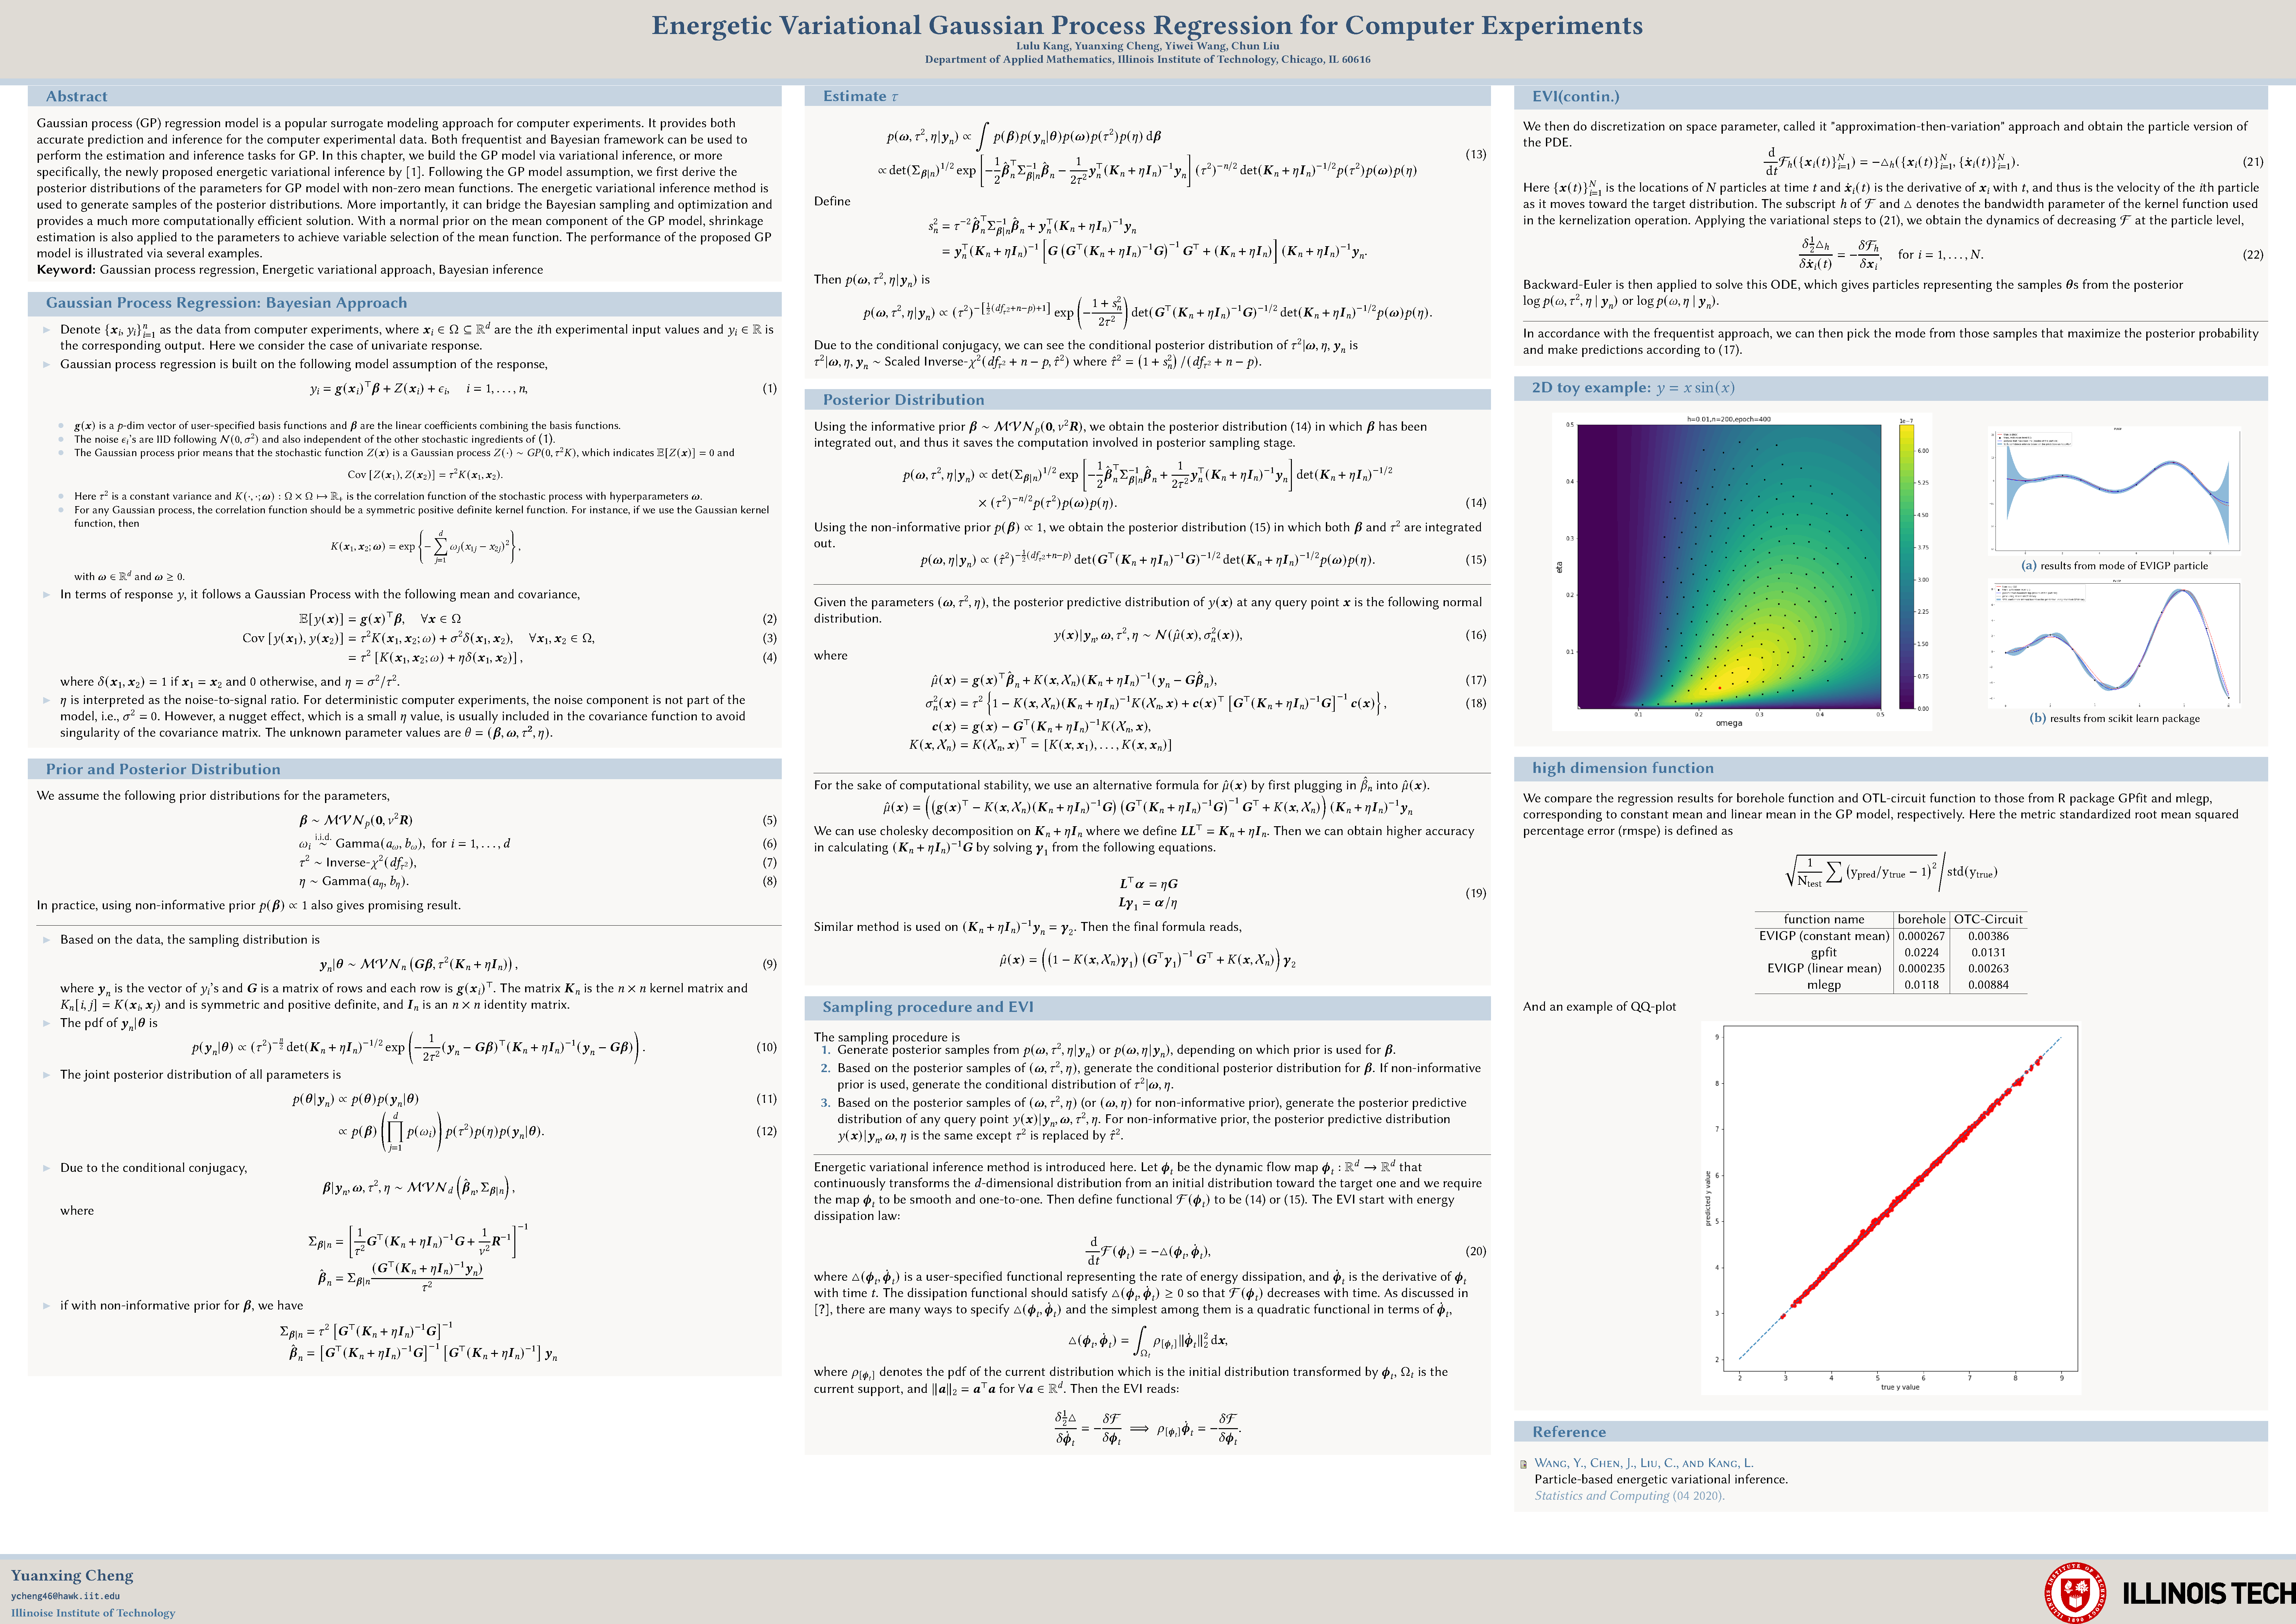
\includegraphics[width=\textwidth]{figures/YXPoster.pdf}
                \label{fig: poster}
            \end{figure}
            \vspace*{-1em}
        \end{column}
    \end{columns}
\end{frame}

\begin{frame}{Some macros}
    \vspace*{-2em}
    \begin{center}
        \begin{tabular}{ll}\\ \hline
            code & usage \\ \hline
            \texttt{\textbackslash begin\{block\}}, \texttt{\textbackslash begin\{theorem\}} & \begin{tabular}[l]{@{}c@{}}to put text in an\\outstanding block\end{tabular}\\
            \texttt{\textbackslash begin\{columns\}} and \texttt{\textbackslash begin\{column\}} & \begin{tabular}[l]{@{}c@{}}to separate a slide\\into columns\end{tabular} \\
            \texttt{\textbackslash usepackage\{multimedia\}} & \begin{tabular}[l]{@{}c@{}}to allow embedding\\multimedia\end{tabular} \\
            \texttt{\textbackslash tableofcontents} & to generate a TOC \\
            \texttt{\textbackslash begin\{center\}} & to center element \\
            \texttt{\textbackslash scalebox} from \texttt{graphicx} package & to adjust equation size\\
            \hline
        \end{tabular}
    \end{center}
\end{frame}

\section{Conclusion}
\begin{frame}{Conclusion}
    \LaTeX\
    \begin{itemize}
        \item A very powerful document preparation system
        \begin{itemize}
            \item Presentation: Slides, Poster
            \item Document: Academic Article, Homework, Report, Resume/CV
        \end{itemize}
        \item Similar to a programming language
        \begin{itemize}
            \item Familiar with its syntax
            \item Need to debug
        \end{itemize}
        \item Some advanced topics with guide on Overleaf
        \begin{itemize}
            \item build your own templates
            \item explore more macros: enumerate, itemize, theorem
            \item type an algorithm
            \item list some code
            \item draw with \texttt{tikz} package
        \end{itemize}
    \end{itemize}
\end{frame}

\section*{ }
\begin{frame}[c]{Q\&A}
	\begin{center}
		\Huge Thank you
	\end{center}
\end{frame}


\begin{frame} [allowframebreaks]\frametitle{References}
    \bibliographystyle{apalike}
    \bibliography{Yuhan}
\end{frame}

\end{document}